%%%%%%%%%%%%%%%%%%%%%%%%%%%%%%%%%%%%%%%%%
% Fancyslides Presentation
% LaTeX Template
% Version 1.0 (30/6/13)
%
% This template has been downloaded from:
% http://www.LaTeXTemplates.com
%
% The Fancyslides class was created by:
% Paweł Łupkowski (pawel.lupkowski@gmail.com)
%
% License:
% CC BY-NC-SA 3.0 (http://creativecommons.org/licenses/by-nc-sa/3.0/)
%
%%%%%%%%%%%%%%%%%%%%%%%%%%%%%%%%%%%%%%%%%

%----------------------------------------------------------------------------------------
%	PACKAGES AND OTHER DOCUMENT CONFIGURATIONS
%----------------------------------------------------------------------------------------

\documentclass{fancyslides}

\usepackage[utf8]{inputenc} % Allows the usage of non-english characters
\usepackage{librebaskerville} % Use the Times font
\usepackage{booktabs} % Allows the use of \toprule, \midrule and \bottomrule in tables
\usepackage[percent]{overpic}
\usepackage{hyperref}
\graphicspath{{images/}} % Location of the slide background and figure files

% Beamer options - do not change
\usetheme{default} 
\setbeamertemplate{navigation symbols}{} % Disable the slide navigation buttons on the bottom of each slide
\setbeamercolor{structure}{fg=\yourowntexcol} % Define the color of titles and fixed text elements (e.g. bullet points)
\setbeamercolor{normal text}{fg=\yourowntexcol} % Define the color of text in the presentation

%------------------------------------------------
% COLORS
% The following colors are predefined in this class: white, black, gray, blue, green and orange

% Define your own color as follows:
\definecolor{cdv}{HTML}{484bb8}

\newcommand{\structureopacity}{0.75} % Opacity (transparency) for the structure elements (boxes and circles)

\newcommand{\strcolor}{cdv} % Set the color of structure elements (boxes and circles)
\newcommand{\yourowntexcol}{white} % Set the text color

\begin{document}

%------------------------------------------------

\fbckg{lichtfeld.jpg} 
\begin{frame}
\misc{
\Huge
Lichtfelddisplays und Hologrammdisplays\\
}
\end{frame}

%------------------------------------------------

\fbckg{stripes.png} 
\begin{frame}
\misc{
\Huge
Inhalt\\
\Large
\begin{flushleft}
\fitem{Menschliche Tiefenwahrnehmung}
\fitem{State of the Art: Stereoskopie}
\fitem{Konzept Lichtfeld}
\fitem{Lichtfelddisplays}
\fitem{Hologramme}
\fitem{Hologrammdisplays}
\end{flushleft}
}
\end{frame}

%------------------------------------------------

\fbckg{stripes.png} 
\begin{frame}
\misc{
\Huge
Menschliche Tiefenwahrnehmung\\
}
\end{frame}

%------------------------------------------------

\fbckg{stripes.png} 
\begin{frame}
\misc{
\Huge
Beschaffenheit des Bildes\\
\Large
\begin{flushleft}
\fitem{Perspektive}
\fitem{Beleuchtung}
\fitem{Schatten}
\fitem{Parallaxe}
\end{flushleft}
}
\end{frame}

%------------------------------------------------

\fbckg{delighted.png} 
\begin{frame}
\end{frame}

%------------------------------------------------

\fbckg{normal.png} 
\begin{frame}
\end{frame}

%------------------------------------------------

\fbckg{stripes.png} 
\begin{frame}
\misc{
\Huge
Physiologische Tiefenwahrnehmung\\
\Large
\begin{flushleft}
\fitem{Akkomodation}
\fitem{Konvergenz}
\fitem{Parallax zwischen Augen}
\end{flushleft}
}
\end{frame}

%------------------------------------------------

\fbckg{stripes.png} 
\begin{frame}
\misc{
\Huge
State of the Art: Stereoskopie\\
}
\end{frame}

%------------------------------------------------

\fbckg{stripes.png} 
\begin{frame}
\misc{
\Huge
Stereoskopie: \\
\Large
\begin{flushleft}
\fitem{Idee: jedes Auge bekommt ein eigenes Bild}
\fitem{Anaglyph}
\fitem{Polarisation}
\fitem{Shutter}
\fitem{Autosteroskopie}
\end{flushleft}
}
\end{frame}

%------------------------------------------------

\fbckg{stripes.png} 
\begin{frame}
\misc{
\Huge
Problem:\\
\Large
\begin{flushleft}
\fitem{Verursacht häufig Kopfschmerzen}
\fitem{Wirkt ermüdend}
\fitem{Beeinträchtigung der Entwicklung bei Kindern?}
\fitem{$\implies$ Nintendo empfiehlt Benutzung erst ab 7 Jahren}
\end{flushleft}
}
\end{frame}

%------------------------------------------------

\fbckg{stripes.png} 
\begin{frame}
\misc{
\Huge
Hauptgrund: Konflikt zwischen Akkomodation und Konvergenz \\
}
\end{frame}

%------------------------------------------------

\fbckg{stripes.png} 
\begin{frame}
\misc{
\Huge
Akkomodation:\\
\Large
\begin{center}
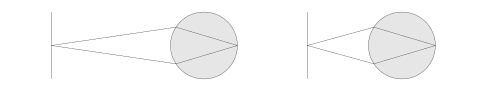
\includegraphics[scale=0.25]{akkomodation.eps}
\end{center}
}
\end{frame}

%------------------------------------------------

\fbckg{stripes.png} 
\begin{frame}
\misc{
\Huge
Konvergenz:\\
\Large
\begin{center}
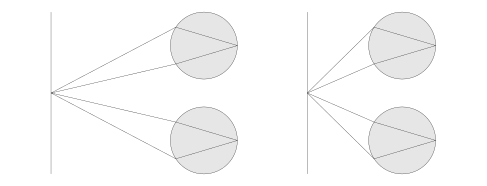
\includegraphics[scale=0.25]{konvergenz.eps}
\end{center}
}
\end{frame}

%------------------------------------------------

\fbckg{stripes.png} 
\begin{frame}
\misc{
\Huge
Naheinstellungstrias:\\
\Large
\begin{flushleft}
\fitem{Pupillenöffnung, Akkomodation und Konvergenz sind fest gekoppelt}
\fitem{Neurophysiologischer Regelkreis}
\end{flushleft}
}
\end{frame}

%------------------------------------------------

\fbckg{stripes.png} 
\begin{frame}
\misc{
\Huge
Akkomodationskorrektur:\\
\Large
\begin{flushleft}
\fitem{Zusätzlich: Akkomodation wird durch Schärfe des Bildes beeinflusst}
\fitem{Solange das Bild scharf genug bleibt bestimmt die Konvergenz die Akkomodation}
\fitem{Ist das Bild trotzdem unscharf wird die Akkomodation korrigiert}
\end{flushleft}
}
\end{frame}

%------------------------------------------------

\fbckg{stripes.png} 
\begin{frame}
\misc{
\Huge
Konflikt:\\
\Large
\begin{center}
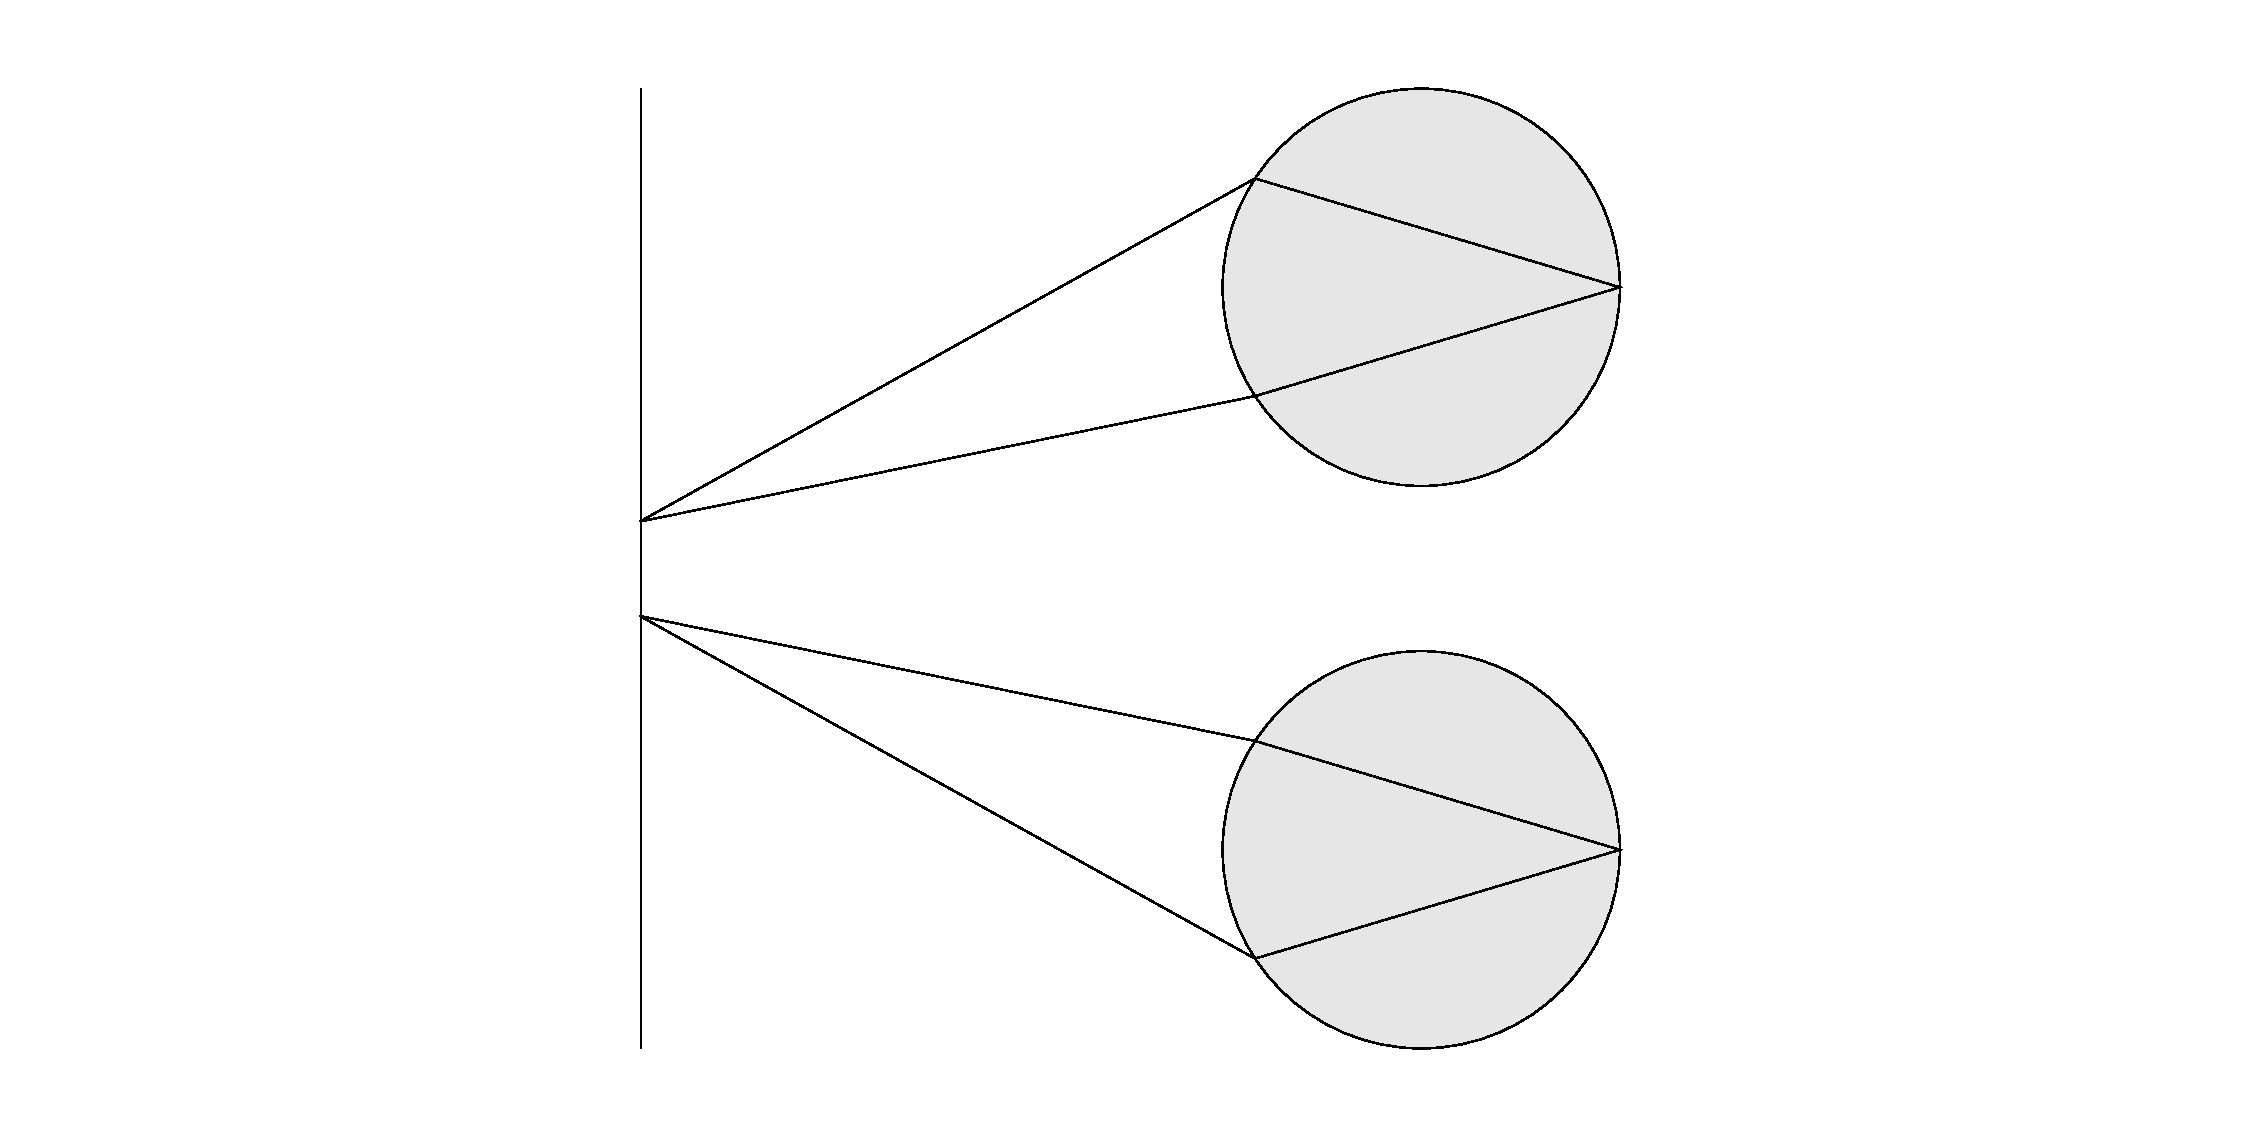
\includegraphics[scale=0.25]{konflikt.eps}
\end{center}
}
\end{frame}

%------------------------------------------------

\fbckg{stripes.png} 
\begin{frame}
\misc{
\Huge
Konflikt:\\
\Large
\begin{flushleft}
\fitem{Beim stereoskopischen Display gibt es einen Konflikt}
\fitem{Im schlimmsten Fall führt das zu oszillierender Akkomodation}
\end{flushleft}
}
\end{frame}

%------------------------------------------------

\fbckg{stripes.png} 
\begin{frame}
\misc{
\Huge
Konzept: Lichtfeld\\
}
\end{frame}

%------------------------------------------------

\fbckg{stripes.png} 
\begin{frame}
\misc{
\Huge
4D Lichtfeld:\\
\Large
\begin{flushleft}
\fitem{2-dimensionale Fläche}
\fitem{In jedem Punkt ein Bündel an Farbwerten}
\fitem{Farbe abhängig von der Richtung}
\end{flushleft}
}
\end{frame}

%------------------------------------------------

\fbckg{stripes.png} 
\begin{frame}
\misc{
\Huge
Vorteile Lichtfeld:\\
\Large
\begin{flushleft}
\fitem{Nicht von einem Fenster unterscheidbar}
\fitem{Perspektive ändert sich mit Betrachterposition}
\fitem{Fokussierung auf virtuelle Ebene}
\end{flushleft}
}
\end{frame}

%------------------------------------------------

\fbckg{stripes.png} 
\begin{frame}
\misc{
\Huge
Geschichte Lichtfeldfotografie:\\
\Large
\begin{flushleft}
\fitem{Bereits 1908 von Gabriel Lippmann vorgeschlagen}
\fitem{Bald darauf erste Prototypen erstellt}
\fitem{Lumière hielt ein Patent für ein Lichtfeldsystem}
\end{flushleft}
}
\end{frame}

%------------------------------------------------

\fbckg{stripes.png} 
\begin{frame}
\misc{
\Huge
Aufbau Lichtfeldkameras:\\
\Large
\begin{flushleft}
\fitem{Linsenarray/Lochgitter vor dem Sensor}
\fitem{Kamera bewegen, mehrere Fotos}
\fitem{Mehrere Kameras}
\\
\includegraphics[scale=0.1]{lytro.jpg} \,
\includegraphics[scale=0.3]{lytro-illum.jpg} \,
\includegraphics[scale=0.12]{camera-array.png} \,
\includegraphics[scale=0.5]{camera-plane-annotated-s.png}
\end{flushleft}
}
\end{frame}

%------------------------------------------------

\fbckg{stripes.png} 
\begin{frame}
\misc{
\Huge
Aufbau Lichtfelddisplays:\\
\Large
\begin{flushleft}
\fitem{Linsenarray/Lochgitter vor dem Display}
\fitem{Gerichtete Hintergrundbeleuchtung}
\fitem{2 Displays hintereinander}
\\
\includegraphics[scale=0.08]{nvidia-neld} \,
\includegraphics[scale=0.1]{red-hydrogen.jpg} \,
\includegraphics[scale=0.17]{LightFieldStereoscope_HMDSchematic.jpg} \,
\end{flushleft}
}
\end{frame}

%------------------------------------------------

\fbckg{lichtfeld.jpg} 
\begin{frame}
\end{frame}

%------------------------------------------------

\fbckg{factored-lightfield.png} 
\begin{frame}
\end{frame}

%------------------------------------------------

\fbckg{stripes.png} 
\begin{frame}
\misc{
\Huge
\href{https://www.youtube.com/watch?v=YJdMPUF8cDM&t=2m11s}{Video}
}
\end{frame}

%------------------------------------------------

\fbckg{stripes.png} 
\begin{frame}
\misc{
\Huge
Desktop Displays:\\
\Large
\begin{flushleft}
\fitem{Problem: Um Akkomodation auf virtuelle Ebene zu ermöglichen muss Winkelauflösung sehr hoch sein}
\fitem{Zusätzlich möchte man einen großen Winkelbereich abdecken}
\fitem{schwierig vereinbar}
\end{flushleft}
}
\end{frame}

%------------------------------------------------

\fbckg{stripes.png} 
\begin{frame}
\misc{
\Huge
Head-Mounted Displays:\\
\Large
\begin{flushleft}
\fitem{Augen bewegen sich nicht relativ zum Display, daher braucht man geringeren Winkelbereich abdecken}
\fitem{Keine weitere Optik nötig um optische Weglänge zu erhöhen, daher kompakte Bauweise}
\end{flushleft}
}
\end{frame}

%------------------------------------------------

\fbckg{stripes.png} 
\begin{frame}
\misc{
\Huge
Vorteile Lichtfelddisplays:\\
\Large
\begin{flushleft}
\fitem{Einfache Bauweise}
\fitem{trotzdem recht gute Ergebnisse}
\fitem{Stereoskopischen Displays überlegen}
\fitem{Rechenaufwand überschaubar, wenn auch deutlich höher als bei Stereoskopie}
\end{flushleft}
}
\end{frame}

%------------------------------------------------

\fbckg{stripes.png} 
\begin{frame}
\misc{
\Huge
Nachteile Lichtfelddisplays:\\
\Large
\begin{flushleft}
\fitem{Es wird sehr hohe Auflösung benötigt}
\fitem{Wird die Auflösung zu hoch treten vermehrt Beugungsfehler auf}
\end{flushleft}
}
\end{frame}

%------------------------------------------------

\fbckg{stripes.png} 
\begin{frame}
\misc{
\Huge
Hologramme $\neq$ Volumetrische Displays\\
\vspace{10mm}
\includegraphics[scale=0.75]{Contest3.jpg} \qquad
\includegraphics[scale=0.3]{star-wars-volumetrisch.png}
}
\end{frame}

%------------------------------------------------

\fbckg{stripes.png} 
\begin{frame}
\misc{
\Huge
Geschichte der Hologramme\\
\Large
\begin{flushleft}
\fitem{Entwickelt von Dennis Gabor in den späten 40ern}
\fitem{Erst seit der Entwicklung des Lasers in den 60ern praktikabel}
\end{flushleft}
}
\end{frame}

%------------------------------------------------

\fbckg{stripes.png} 
\begin{frame}
\misc{
\Huge
Idee von Hologrammen:\\
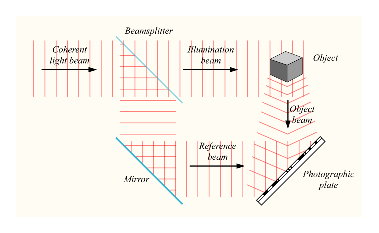
\includegraphics[scale=1.3]{Holograph-record.eps} \,
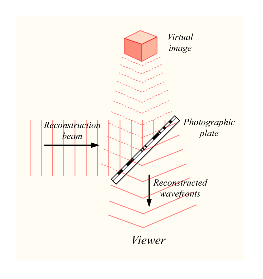
\includegraphics[scale=1.3]{Holography-reconstruct.eps}
}
\end{frame}

%------------------------------------------------

\fbckg{stripes.png} 
\begin{frame}
\misc{
\Huge
Fresnel-Zonenplatte:\\
\vspace{5mm}
\includegraphics[scale=0.15]{Zonenplatte_Cosinus.png}\,
}
\end{frame}

%------------------------------------------------

\fbckg{stripes.png} 
\begin{frame}
\misc{
\Huge
Fresnel-Zonenplatte:\\
\Large
\begin{flushleft}
\fitem{Komplett flach}
\fitem{Verändert Amplitude und Phase des Lichts}
\fitem{Wirkt auf kohärentes Licht wie eine Linse}
\fitem{Brennweite hängt von der Wellenlänge des Lichts ab}
\fitem{Änderung der Brennweite durch Skalierung}
\end{flushleft}
}
\end{frame}

%------------------------------------------------

\fbckg{stripes.png} 
\begin{frame}
\misc{
\Huge
Digitale Holographie:\\
\Large
\begin{flushleft}
\fitem{Überlagerung von Fresnel-Zonenplatten berechnen}
\fitem{Auflösung bestimmt wie stark das Licht abgelenkt werden kann}
\fitem{Entsprechende LCD-Displays steuern Phase des Lichts}
\fitem{Entweder nur Phase, oder (besser) Phase und Amplitude}
\end{flushleft}
}
\end{frame}

%------------------------------------------------

\fbckg{stripes.png} 
\begin{frame}
\misc{
\Huge
Zonenplatten überlagern:\\
\Large
\vspace{5mm}
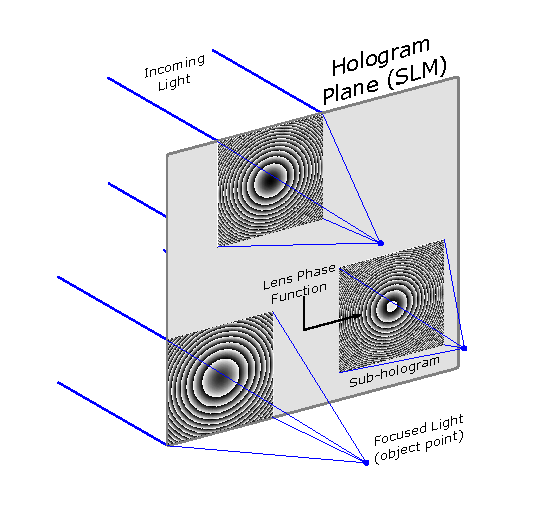
\includegraphics[scale=0.6]{holo_author.eps} \,
\includegraphics[scale=0.21]{digitales-hologramm.eps} \,
}
\end{frame}

%------------------------------------------------

\fbckg{colormap.png} 
\begin{frame}
\end{frame}

%------------------------------------------------

\fbckg{depthmap.png} 
\begin{frame}
\end{frame}

%------------------------------------------------

\fbckg{phasemap.png} 
\begin{frame}
\end{frame}

%------------------------------------------------

\fbckg{ampmap.png} 
\begin{frame}
\end{frame}

%------------------------------------------------

\fbckg{stripes.png}
\begin{frame}
\misc{
\Huge
\href{https://www.youtube.com/watch?v=lN4tFV16mU8}{Video}
}
\end{frame}

%------------------------------------------------

\fbckg{stripes.png} 
\begin{frame}
\misc{
\Huge
Vorteile Hologrammdisplays:
\Large
\begin{flushleft}
\fitem{Lichtfeld kann sehr exakt rekonstruiert werden}
\fitem{Es wird weniger Auflösung benötigt als bei Lichtfelddisplays}
\fitem{Beugung ist kein Fehler sondern ein Feature}
\fitem{Auflösung daher nur durch Displaytechnologie begrenzt}
\end{flushleft}
}
\end{frame}

%------------------------------------------------

\fbckg{stripes.png} 
\begin{frame}
\misc{
\Huge
Nachteile Hologrammdisplays:
\Large
\begin{flushleft}
\fitem{Sehr hoher Rechenaufwand}
\fitem{Spezielle Displays benötigt}
\fitem{Farbe muss über Zeitmultiplexing realisiert werden}
\fitem{Hohe Auflösung benötigt}
\end{flushleft}
}
\end{frame}

%------------------------------------------------

\fbckg{stripes.png} 
\begin{frame}
\pointedsl{Fragen?}
\end{frame}

%------------------------------------------------

\fbckg{stripes.png} 
\begin{frame}
\misc{
\Huge
Quellen/Weitere Infos\\
\small
\begin{flushleft}
\fitem{\href{https://doi.org/10.1016/j.displa.2007.09.004}{Visual fatigue caused by viewing stereoscopic motion images: Background, theories, and observations}}
\fitem{\href{https://doi.org/10.1016/0042-6989(77)90211-5}{Dependence of accommodation response on the spatial frequency spectrum of the observed object}}
\fitem{\href{https://doi.org/10.1002/jsid.303}{Measurement of the lens accommodation in viewing stereoscopic displays}}
\fitem{\href{http://research.nvidia.com/sites/default/files/publications/c121-f121_199-a18-paperfinal-v3.pdf}{Perceptually-Guided Foveation for Light Field Displays}}
\fitem{\href{http://research.nvidia.com/sites/default/files/pubs/2013-11_Near-Eye-Light-Field/NVIDIA-NELD.pdf}{Near-Eye Light Field Displays}}
\fitem{\href{http://cfg.mit.edu/sites/cfg.mit.edu/files/near-eye-light-field-holographic-rendering.pdf}{Near-eye Light Field Holographic Rendering with Spherical Waves for Wide Field of View Interactive 3D Computer Graphics}}
\fitem{\href{http://www.computationalimaging.org/wp-content/uploads/2015/06/TheLightFieldStereoscope-SIGGRAPH2015.pdf}{The Light Field Stereoscope}}
\fitem{\href{http://research.nvidia.com/sites/default/files/pubs/2017-11_Near-Eye-Varifocal-Augmented//AksitEtAl_SiggraphAsia2017_Near\%20eye\%20varifocal\%20augmented\%20reality\%20display\%20using\%20see-through\%20screens.pdf}{Near-Eye Varifocal Augmented Reality Display using See-Through Screens}}
\fitem{\href{https://www.microsoft.com/en-us/research/wp-content/uploads/2017/05/holo_author.pdf}{Holographic Near-Eye Displays for Virtual and Augmented Reality}}
\end{flushleft}
}
\end{frame}

%------------------------------------------------

\end{document}
